\documentclass[11pt]{amsart}
\usepackage{geometry}                
\geometry{letterpaper}                   

\usepackage{graphicx}
\usepackage{amssymb}
\usepackage{epstopdf}
\usepackage{tikz}

\DeclareGraphicsRule{.tif}{png}{.png}{`convert #1 `dirname #1`/`basename #1 .tif`.png}
\pagenumbering{gobble}

\title{Advanced Encryption Standard (AES)}
\author{Eric Gunn}

\begin{document}
\maketitle
\begin{figure}
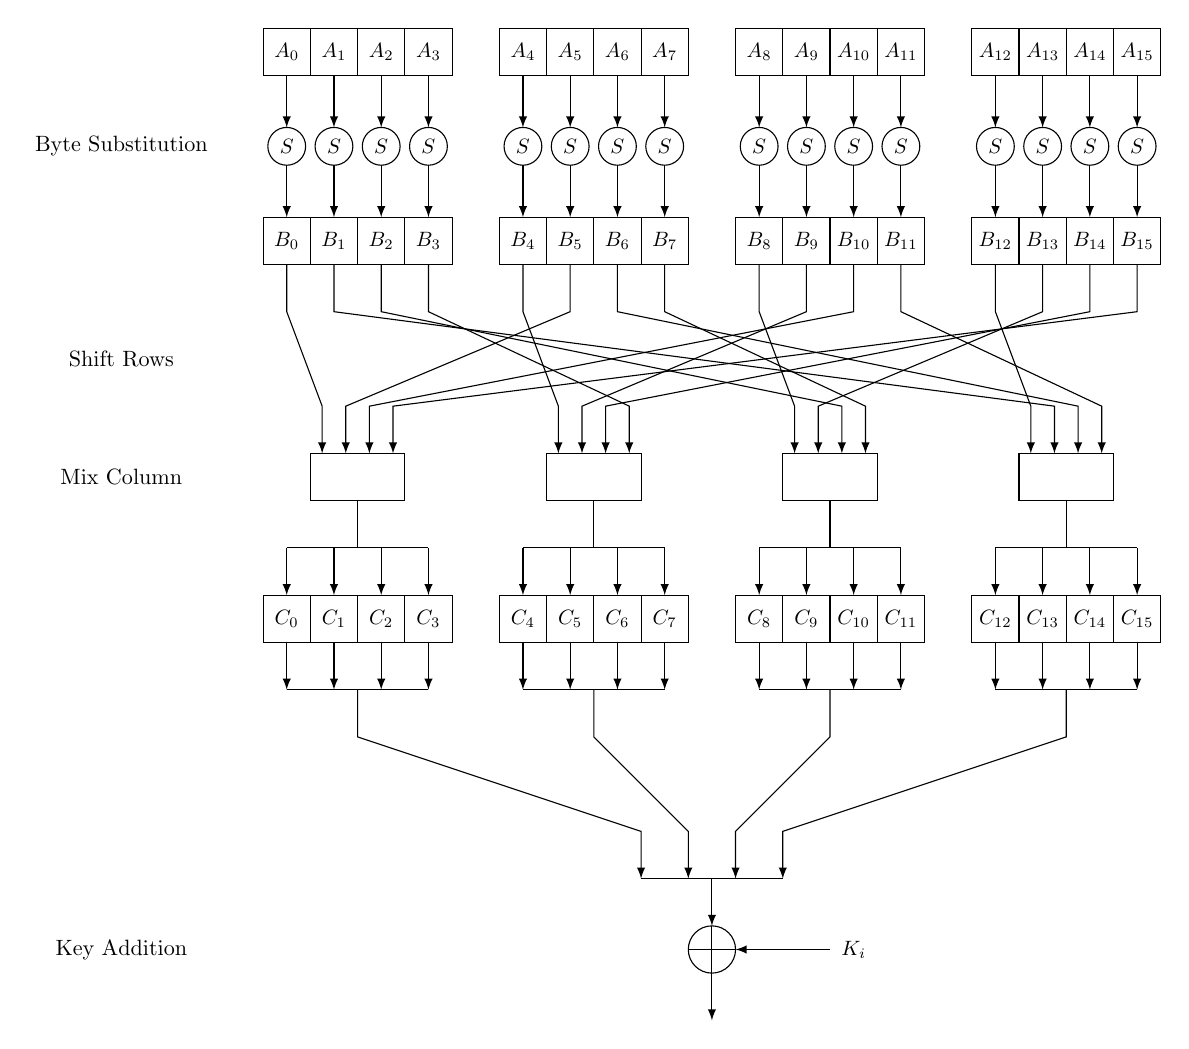
\begin{tikzpicture}[scale=0.6]
%\draw [help lines] (0,0) grid (25,25);

\foreach \x in {6,...,25}{
	\draw (\x,22)--(\x,23);
	\draw (\x,18)--(\x,19);
	\draw (\x,10)--(\x,11);
}
\foreach \x in {6,11,16,21}{
	\draw (\x,22) rectangle (\x+4,23);
	\draw (\x,18) rectangle (\x+4,19);
	\draw (\x,10) rectangle (\x+4,11);
	\draw (\x+2,13)--(\x+2,12);
	\draw (\x+0.5,12)--(\x+3.5,12);
	\draw (\x+0.5,9)--(\x+3.5,9);
	\begin{scope}[>=latex]
		%B0, B4, B8, B12 arrows
		\draw [->] (\x+0.5,18)--(\x+0.5,17)--(\x+1.25,15)--(\x+1.25,14);
	\end{scope}
}
\foreach \x in {6,11,16}{
	\begin{scope}[>=latex]
		%B5, B9, B13 arrows
		\draw [->] (\x+6.5,18)--(\x+6.5,17)--(\x+1.75,15)--(\x+1.75,14);
		%B3, B7, B11 arrows
		\draw [->] (\x+3.5,18)--(\x+3.5,17)--(\x+7.75,15)--(\x+7.75,14);
	\end{scope}
}
\foreach \x in {6,11}{
	\begin{scope}[>=latex]
		%B10, B14 arrows
		\draw [->] (\x+12.5,18)--(\x+12.5,17)--(\x+2.25,15)--(\x+2.25,14);
		%B2, B6 arrows
		\draw [->] (\x+2.5,18)--(\x+2.5,17)--(\x+12.25,15)--(\x+12.25,14);
	\end{scope}
}
\begin{scope}[>=latex]
	%B1 arrow
	\draw [->] (7.5,18)--(7.5,17)--(22.75,15)--(22.75,14);
	%B15 arrow
	\draw [->] (24.5,18)--(24.5,17)--(8.75,15)--(8.75,14);
	%C0-C3 arrow
	\draw [->] (8,9)--(8,8)--(14,6)--(14,5);
	%C4-C7 arrow
	\draw [->] (13,9)--(13,8)--(15,6)--(15,5);
	%C8-C11 arrow
	\draw [->] (18,9)--(18,8)--(16,6)--(16,5);
	%C12-C15 arrow
	\draw [->] (23,9)--(23,8)--(17,6)--(17,5);
	%K arrow
	\draw [<-] (16,3.5)--(18,3.5);
\end{scope}

%K label
\node [scale=0.75] at (18.5,3.5) {$K_{i}$};
%horizontal line above XOR
\draw (14,5)--(17,5);
%XOR
\draw (15.5,3.5) circle [radius=0.5];
\draw (15,3.5)--(16,3.5);
\draw (15.5,4)--(15.5,3);
%XOR arrows
\foreach \x in {2,4}{
	\begin{scope}[>=latex]
		\draw [<-] (15.5,\x)--(15.5,\x+1);
	\end{scope}
}
%labels
\node [scale=0.8] at (3,20.5) {Byte Substitution};
\node [scale=0.8] at (3,16) {Shift Rows};
\node [scale=0.8] at (3,13.5) {Mix Column};
\node [scale=0.8] at (3,3.5) {Key Addition};
\foreach \x [count=\xi] in {6.5,...,9.5,11.5,12.5,...,14.5,16.5,17.5,...,19.5,21.5,22.5,...,24.5}{
	\pgfmathsetmacro\result{int(\xi - 1)} %subtract 1 from \xi and set to \result, cast as int
	\node [scale=0.75] at (\x,22.5) {$A_{\result}$};
	\node [scale=0.75] at (\x,18.5) {$B_{\result}$};
	\node [scale=0.75] at (\x,10.5) {$C_{\result}$};
	\draw (\x,20.5) circle [radius=0.4];
	\node [scale=0.75] at (\x,20.5) {$S$};
	\begin{scope}[>=latex]
		\draw [->] (\x,22)--(\x,20.9);
		\draw [->] (\x,20.1)--(\x,19);
		\draw [->] (\x,12)--(\x,11);
		\draw [->] (\x,10)--(\x,9);
	\end{scope}
}
\foreach \x in {7,12,17,22}{
	\draw (\x,13) rectangle (\x+2,14);
}
\end{tikzpicture}
\caption {AES round function for rounds $1, 2,\dotsc,n_{r-1}$}
\end{figure}
\end{document}  